\documentclass{school-22.211-notes}
\date{March 19, 2012}

\begin{document}
\maketitle

\lecture{One-Group Diffusion: Criticality Problem}
\topic{Helmholtz Equation}
We start with the one-group diffusion equation,
\eqn{ -\divergence D(\vecr) \gradient \phi(\vecr) + \Sigma_a(\vecr) \phi(\vecr) = \frac{1}{\keff} \nu \Sigma_f(\vecr) \phi(\vecr) }
Assume homogeneous material, that is, spatial constant cross section,
\eqn{ -D \laplacian \phi(\vecr) + \Sigma_a \phi(\vecr) = \frac{1}{\keff} \nu \Sigma_f \phi(\vecr) }
Rearranging and defining a buckling term, 
\eqn{ \laplacian \phi(\vecr) + \underbrace{\frac{ \frac{\nu \Sigma_f}{\keff} - \Sigma_a}{D} }_{B^2} \phi(\vecr) = 0 }
We obtain a classic Helmholtz Equation,
\eqn{ \boxed{\laplacian \phi(\vecr) + B_m^2 \phi(\vecr) = 0 } }
Helmholtz Equation implies that,
\eqn{ B_m^2 = - \frac{\laplacian \phi(\vecr)}{\phi(\vecr)} }
Notice,
\begin{enumerate}
\item Since $B_m^2$ is a constant, that is to say $\frac{\laplacian \phi(\vecr)}{\phi(\vecr)}$ is a constant, that is to say $\phi(\vecr)$ has a constant curvature. 
\item Material buckling: 
  \eqn{ B_m^2 = \frac{\frac{\nu \Sigma_f}{\keff} - \Sigma_a}{D} }
  which matches geometry buckling, 
  \eqn{ \keff = \frac{\nu \Sigma_f}{DB_g^2 + \Sigma_a} }
  where $DB^2_g$ is the leakage per unit volume per unit flux. Notice $\keff$ does not depend on volume or flux. 

\item Critical buckling: when a system is critical, the material buckling is uniquely determined by cross sections, 
  \eqn{ B_m^2 = \frac{\nu \Sigma_f - \Sigma_a}{D} = \frac{\frac{\nu \Sigma_f}{\Sigma_a} - 1}{\frac{D}{\Sigma_a}} = \frac{\kinf - 1}{M^2} }
  \hi{Migration area} $M^2 = \frac{D}{\Sigma_a}$ is a measurement of the amount of travelling before absorption. 

\item Solutions exist only for certain values of the buckling such that the flux is everywhere positive and vanishing on outer (or extrapolated) surfaces; we define these unique values as `geometrical buckling' $B_g^2$. The allowable values of geometrical buckling that satisfy the boundary conditions are uniquely determined reactor geometry.

\item For a criticality problem, we can solve find the $B^2$ such that the system is critical. Hence giving geometry, only certain materials would make the system critical; given material, only certain geometries would make the system critical. That is, given a reactor, it would be critical if and only if the material and the geometry satisfy,
  \eqn{ B_g^2 = B_m^2} 

\item Solution only exists when $\kinf > 1$ (exception: if there is external source, $\kinf$ can be less than 1 and the system is still critical). 
\end{enumerate}

Talbe~\ref{simple-geometry-laplacian} lists a couple of one group homogeneous geometry Laplacians. 
\begin{table}
  \centering
  \begin{tabular}{|l|l|} \hline
    Slab & $\dphidxn2 + B^2 \phi(x) = 0$ \\ \hline
    Sphere & $\dphidrn2 + \frac{2}{r} \dphidr + B^2 \phi(r) = 0$ \\ \hline
    Infinite Cylinder & $\dphidrn2 + \frac{1}{r} \dphidr + B^2 \phi(r) = 0$ \\ \hline
    Finite Cylinder & $\dphidrn2 + \frac{1}{r} \dphidr + \dphidzn2 + B^2 \phi(r,z) = 0$ \\ \hline
    Cartesian & $\dphidxn2 + \dphidyn2 + \dphidzn2 + B^2 \phi(x,y,z) = 0$ \\ \hline
  \end{tabular}
\caption{Simple Geometry Laplacians} \label{simple-geometry-laplacian}
\end{table}




\clearpage
\topic{Critical 1D Slab}
 Consider a 1D slab $\in  \left[- \frac{L_0}{2}, \frac{L_0}{2} \right]$:
  \eqn{ \dphidxn2 + B^2 \phi (x) &= 0, &\phi(x) &= A \cos (Bx) + C \sin(Bx) }
BCs: $\phi(\pm L/2) = 0$, $\frac{L}{2} = \frac{L_0}{2} + 0.711 \lambda_{tr}$. Two equations two unknowns, 
  \eqn{ \left[ \begin{array}{cc} \cos(BL/2) & \sin(BL/2) \\ \cos(BL/2) & -\sin(BL/2) \end{array} \right] \left[ \begin{array}{cc} A \\ C \end{array} \right] = 0 }
  Set the determinant to be zero, we get $-2 \cos (BL/2) \sin (BL/2) = 0$. There are two possibilities: 
\eqn{ B_n&= \frac{n\pi}{L}  & \phi(x) &= \left\{ 
  \begin{array}{cc} 
    A_n \cos (B_n x) & n=1,3,5, \cdots \\
    A_n \sin (B_n x) & n=2,4,6, \cdots 
  \end{array} \right. }
But in order for $\phi(x) \ge 0$ everywhere, only $n=1$ is possible; that is, 
\eqn{ \phi(x) = A \cos \frac{\pi x}{L} }
and the criticality condition implies that, 
\eqn{ \frac{\nu \Sigma_f - \Sigma_a}{D}  = \left( \frac{\pi}{L} \right)^2 }

\clearpage
\topic{Critical Finite Cube}
Consider a finite cube with the dimensions $-a/2 \le x \le a/2, -b/2 \le y \le b/2, -c/2 \le z \le c/2$. The Helmholtz equation is,
\eqn{ \pphipxn2 + \pphipyn2 + \pphipzn2 + B^2 \phi = 0}
Assume separation of variables,
\eqn{ \phi(x,y,z) = X(x) Y(y) Z(z) }
\eqn{ \dXdxn2 + B_x^2 X &= 0, &\dYdyn2 + B_y^2 Y &= 0, &\dZdzn2 + B_z^2 Z &=0}
The solution is, 
\eqn{ \phi &= A \cos \left( \frac{\pi x}{L_x} \right)\cos \left( \frac{\pi y}{L_y} \right)\cos \left( \frac{\pi z}{L_z} \right) ,  &B^2 &= \left(\frac{\pi}{a}\right)^2 + \left(\frac{\pi}{b}\right)^2 + \left(\frac{\pi}{c}\right)^2 }

\clearpage
\topic{Critical Finite Cylinder} 
Consider a finite cylinder from $-H/2$ to $H/2$ with radius $R$. We assume azmimuthal symmetry of Helmholtz Equation, 
\eqn{\frac{1}{r} \ddr \left( r \pphipr\right) + \pphipzn2 + B^2 \phi = 0 }
Assume separation of variables,
\eqn{ \phi(r,z) = R(r) Z(z) }
We plut the sepration of variables into the Helmholtz Equation, break $B^2 = B_r^2 + B_z^2$, and we get two equations one for each direction, 
\eqn{ \frac{1}{R} \left( \dRdrn2 + \frac{1}{r} \dRdr \right) + B_r^2 = 0 }
\eqn{ \dZdzn2 + B_z^2 Z = 0 }
In $r$ direction, we can consider an infinite cylinder, 
\eqn{ R(r) &= A_1 J_0 (B_r r), & B_r&= \frac{2.405}{R} }
In $z$ direction, we can consider an infinite slab,
\eqn{ Z(z) &= A_2 \cos(B_z z), & B_z &= \frac{\pi}{H} } 
We combine the two directions,
\eqn{ \phi(r,z) &= A J_0 \left( \frac{2.405}{R} r\right) \cos \left( \frac{\pi z}{H} \right), &B^2 &= B_r^2 + B_z^2 = \left( \frac{2.405}{R} \right)^2 + \left( \frac{\pi}{H} \right)^2 }
Problems with less than one direction that is non-homogeneous can be solved this way with separation of variables.

\clearpage
\topic{Critical Reflected Slab Reactor}\label{critical-reflected-slab}
Consider a critical reflected slab reactor as in Figure~\ref{reflected-slab}. 
\begin{figure}[ht]
  \centering
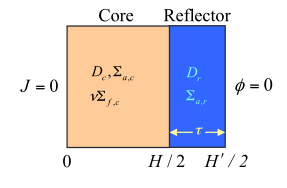
\includegraphics[width=2.5in]{images/dfs/reflected-slab.png}
\caption{A Critical Reflected Slab Geometry} \label{reflected-slab}
\end{figure}
The Helmholtz equations for the two regions are,
\eqn{-D^c \laplace \phi^c + \Sigma_a^c \phi^c &= \frac{1}{\keff} \nu \Sigma_f^c \phi^c,  &-D^r \laplace \phi^r + \Sigma_a^r \phi^r &= 0 }
\eqn{ B^2 &= \frac{\frac{\kinf}{\keff} - 1}{L_c^2}, & \kappa^2 &= \frac{1}{L_r^2} = \frac{\Sigma_a^r}{D^r} = -B_{m,r}^2 }
\eqn{ \laplace \phi^c + B^2 \phi^c &= 0, &\laplace \phi^r - \kappa^2 \phi^r &= 0}
The solutions are in the forms of,
\eqn{ \phi^c(x) &= C_1 \cos(Bx) + C_2 \sin(Bx), &\phi^r(x) &= C_3 \cosh(\kappa x) + C_4 \sinh (\kappa x) }
BC1: reflective boudnary condition at $x=0$, BC2: zero flux at reflector surface, 
\eqn{ J^c(0) &= 0 \Rightarrow C_2 = 0, & \phi(H'/2) &= 0 \Rightarrow C_3 = 0} 
We have: 
\eqn{ \phi^c (x) &= C_1 \cos (Bx), & \phi^r (x) &= C_4' \sinh[\kappa(H'/2 - x)] }
Apply two interface conditions: 
\eqn{ \phi^c (H/2) &= \phi^r (H/2), & J^c(H/2) &= J^r (H/2) }
which can be written in the matrix form, 
\begin{align}
\left[ \begin{array}{cc}
\cos (BH/2) & -\sinh(\kappa \tau) \\
D^c B \sin(BH/2) & -D^r \kappa \cosh(\kappa \tau) 
\end{array} \right] 
\left[ \begin{array}{c} 
C_1 \\ C_4' \end{array} \right] = 0
\end{align}
We define the reflector thickness $\tau = \frac{H' - H}{2}$, then the coefficients can be solved,
\eqn{ C_1 &= \phi^c (0), & C_4' &= C_1 \frac{\cos (BH/2)}{\sinh(\kappa \tau) } }
which gives us the criticality condition,
\eqn{ D^c B \tan \left(\frac{B H}{2} \right) = D^r \kappa \coth (\kappa \tau) }
Interpretation:
\begin{enumerate}
\item Since $B$ is defined with $\keff$, 
  \eqn{ B^2 = \frac{\frac{\kinf}{\keff} - 1}{L^2} }
  we need to satisty an expression between $\keff$ and $H$. We can either,
  \begin{enumerate}
  \item Given $H$, search for the $\keff$ that satisfies the equivalence;
  \item Given $\keff$, search for the $H$ that satisfies the equivalence,
    \eqn{H = \frac{2}{B_m} \tan^{-1} \left[ \frac{D^r \kappa}{D^c B_m} \coth (\kappa \tau) \right] }
    That is, as $H \down, \tau \up$. For large $\tau$, like $\kappa \tau > 3, \coth (\kappa \tau) \to 1$, the smallest $H$ to reach criticality is,
    \eqn{H = \frac{2}{B_m} \tan^{-1} \left[ \frac{D^r \kappa}{D^c B_m} \right] }
  \end{enumerate}
\item Critical dimension is reduced by the presence of the reflector: 
\eqn{   s = \frac{\tilde{H}}{2} - \frac{H}{2}   = \frac{1}{B_m} \left\{ \frac{\pi}{2} - \tan^{-1} \left[ \frac{D^r \kappa}{D^c B_m} \coth(\kappa \tau) \right] \right\} }
\eqn{   \tan\left[ \frac{\pi}{2} - \tan^{-1} x \right] &= \cot [\tan^{-1} x ] = \frac{1}{\tan[\tan^{-1} x]} = \frac{1}{x}, & \frac{\pi}{2} - \tan^{-1} x &= \tan^{-1} \left( \frac{1}{x} \right) }
\eqn{  \Aboxed{ s &= \frac{1}{B_m} \tan^{-1} \left[ \frac{D^c B_m}{D^r \kappa} \tanh(\kappa \tau) \right] } }
\item For larger cores, $B_m \to 0$ and $\tan^{-1} x \approx x $, that is, 
\eqn{ s = \frac{D^c}{D^r \kappa} \tanh(\kappa \tau) = \frac{D^c}{D^r} L^r \tanh\left( \frac{\tau}{L^r} \right)  }
That is, 
\begin{align}
  \left\{ \begin{array}{ccc} 
    \tau \ll L^r & s \approx \frac{D^c}{D^r} \tau &  (\tanh x \approx x \mbox{ for }x\ll 1) \\
    \tau \gg L^r & s \approx \frac{D^c}{D^r} L^r &  (\tanh x \approx 1 \mbox{ for }x > 3) 
  \end{array} \right. 
\end{align}
\item For more on reflector saving, see Reuss' Section 6.1.5 (p.173). 
\end{enumerate}


\clearpage
\topic{Summary}
\begin{table}[ht]
  \small
  \makebox[\textwidth][c]{
  \begin{tabular}{|l|l|l|l|} \hline
    Geometry & Diffusion Equation & Flux & Geometrical Buckling \\ \hline
    Slab $\in  \left[- \frac{L}{2}, \frac{L}{2} \right]$ &$\dphidxn2 + B^2 \phi = 0$ & $\phi = A \cos \left( \frac{\pi x}{L} \right)$ & $B^2 = \left( \frac{\pi}{L} \right)^2$ \\ 
    Sphere $\in [0, R]$  & $\dphidrn2 + \frac{2}{r} \dphidr + B^2 \phi = 0$& $\phi= \frac{A}{r} \sin \left( \frac{\pi r}{R} \right)$ & $B^2 = \left( \frac{\pi}{R} \right)^2$ \\
    Cylinder ($z: \infty$) & $\dphidrn2 + \frac{1}{r} \dphidr + B^2 \phi = 0$ & $\phi = A J_0 \left( \frac{2.405 r}{R} \right)$ & $B^2 = \left( \frac{2.405}{R} \right)^2$ \\ 
    Cylinder (z: $\pm H/2$) & $\dphidrn2 + \frac{1}{r} \dphidr + \dphidzn2 + B^2 \phi = 0$ & $\phi = A J_0\left( \frac{2.405 r}{R} \right) \cos \left( \frac{\pi z}{H} \right)$ & $B^2 = \left( \frac{2.405}{R} \right)^2 + \left( \frac{\pi}{H} \right)^2$ \\ 
    Parallelepiped ($\pm \frac{L_i}{2}$) & $\dphidxn2 + \dphidyn2 + \dphidzn2 + B^2 \phi = 0$ & $\phi = A \cos \left( \frac{\pi x}{L_x} \right) \cos \left( \frac{\pi y}{L_y} \right) \cos \left( \frac{\pi x}{L_z} \right)$ & $B^2 = \left( \frac{\pi}{L_x} \right)^2 + \left( \frac{\pi}{L_y} \right)^2 + \left( \frac{\pi}{L_z} \right)^2$ \\ \hline
  \end{tabular}
}
  \caption{One Group Fundamental Mode Eigenvalues and Eigenvectors} \label{eigen-values}
\end{table}
\normalsize

Observations:
\begin{itemize}
\item The lowest node is the only one remains after the source is gone. 
\item For any positive value of materials buckling, there is a unique critical size for each reactor geometry. 
\item Know how to get the critical buckling for different geometries. 
\item Seperation of variables works as long as there is no one more than one direction that is heterogeneous. 
\item Example: know how to find height-to-diameter to minimize leakage. The optimal cylinder has a H/D of around 0.92. 
\end{itemize}

\end{document}
